%------------------ vorlage.tex ------------------------------------------------
%
% LaTeX-Vorlage zur Erstellung von Projektdokumentationen
% im Fachbereich Informatik der Hochschule Trier
%
% Basis: Vorlage 'svmono' des Springer Verlags
% Bearbeiter: Hermann Schloß, Christian Bettinger
%
%-------------------------------------------------------------------------------


%------------------ Präambel ---------------------------------------------------
\documentclass[envcountsame, envcountchap, deutsch]{i-studis}

\usepackage[utf8]{inputenc}

\usepackage[a4paper]{geometry}
\usepackage[english, ngerman]{babel}

\usepackage[pdftex]{graphicx}
\usepackage{epstopdf}

\usepackage{listings}

\usepackage[german, ruled, vlined]{algorithm2e}
\usepackage{amssymb, amsfonts, amstext, amsmath}
\usepackage{array}
\usepackage[skip=10pt]{caption}
\usepackage[usenames, dvipsnames]{color}
\usepackage[pdftex, plainpages=false]{hyperref}
\usepackage{textcomp}

\usepackage{bibgerm}
\bibliographystyle{geralpha}

\usepackage{makeidx}
\usepackage{multicol}
\makeindex

\pagestyle{myheadings}
\setlength{\textheight}{1.1\textheight}

\usepackage{xcolor}
\lstset { %
    language=C++,
    backgroundcolor=\color{black!5}, % set backgroundcolor
    basicstyle= \footnotesize \bfseries ,% basic font setting
	keywordstyle=\color{blue}\bfseries ,
	stringstyle=\color{red}\bfseries ,
	commentstyle=\color{teal}\bfseries ,
	morecomment=[l][\color{magenta}]{\#}
}


%------------------ Manuelle Silbentrennung ------------------------------------
\hyphenation{Ele-men-tar-ob-jek-te ab-ge-tas-tet Aus-wer-tung House-holder-Matrix Least-Squares-Al-go-ri-th-men}


%------------------ Titelseite -------------------------------------------------
\begin{document}

\title{Stripification Tool}
\subtitle{Projekt für das Modul Tool- und Pluginprogrammierung}

\author{Florian Wößner}

\supervisor{Prof. Dr. Christof Rezk-Salama}

\address{Trier}
\submitdate{31.08.2024}

%------------------ Projektart -------------------------------------------------
%\project{Bachelor-Projektarbeit}
%\project{Bachelor-Abschlussarbeit}
%\project{Master-Projektstudium}
%\project{Master-Abschlussarbeit}
%\project{Seminar}
\project{Hausarbeit}

\mytitlepage

%------------------ Vorwort, Kurzfassung, Verzeichnisse ------------------------
\frontmatter
\tableofcontents										% Inhaltsverzeichnis


%------------------ Kapitel ----------------------------------------------------
\mainmatter
\chapter{Einleitung}

Das Ziel dieses Projekts ist es, nach dem Einlesen einer OBJ-Datei, die
enthaltenen Dreiecke in Strips zusammenzufassen und diese effizient zu zeichnen.
Die Technik der Stripification spielt dabei eine zentrale Rolle und bringt
signifikante Vorteile mit sich.
\\
\\
Stripification bezeichnet den Prozess, bei dem Dreiecke eines 3D-Modells in
sogenannte Triangle Strips umgewandelt werden. Ein Triangle Strip ist eine
Sequenz von Vertices, bei der jedes aufeinanderfolgende Dreieck durch Hinzufügen
eines weiteren Vertex definiert wird. Diese Methode reduziert den Speicherbedarf
für die Vertices auf der GPU, da weniger redundante Daten gespeichert werden
müssen. Beispielsweise wird aus den einzelnen Dreiecken mit Vertices (1, 2, 3),
(3, 2, 4) und (3, 4, 5) nach der Stripification der Strip (1, 2, 3, 4, 5). Dies
bedeutet, dass die Vertices 3 und 4 nicht mehrfach gespeichert werden müssen,
was die Effizienz der Speicher- und Renderprozesse erhöht. 
\\
\\
Das Projekt baut auf dem bestehenden Projekt „ObjToVertexBuffer“ auf, das in
einer Übungsstunde bearbeitet wurde. Dieses Ausgangsprojekt stellt bereits einen
OBJ-Datei-Parser zum Einlesen von 3D-Modellen sowie einen fertigen Canvas mit
den passenden Datenstrukturen bereit, was eine solide Basis für die
Weiterentwicklung darstellt.
\\
\\
Zur Erreichung der Projektziele wurden folgende Teilaufgaben definiert und
umgesetzt:
\begin{itemize}
    \item Implementierung des Triangels-to-Strip Konverters
    \item Implementierung des Strip-Zeichners
    \item Allgemeine Anpassung des vorhandenen Codes
    \item Implementierung der Steuerung und einer GUI
\end{itemize}
\hfil \break
Die von mir ergänzten Codeabschnitte sind zur besseren Nachverfolgbarkeit mit
Kommentaren markiert:

\begin{lstlisting}
    // <Florian>
    ...
    // </Florian>
\end{lstlisting}
\chapter{Implementierung des Triangels-to-Strip Konverters}

Die Konvertierung von Dreieckspunkten zu Strips erfolgt in der Methode \break
\lstinline{void Mesh3D::generateStrips()}. Diese Methode führt die Hauptarbeit
bei der Strip-Generierung durch, wie in den Vorlesungsfolien beschrieben
(Abbildung \ref{fig:SGI}). 

\begin{figure}[ht]
    \centering
    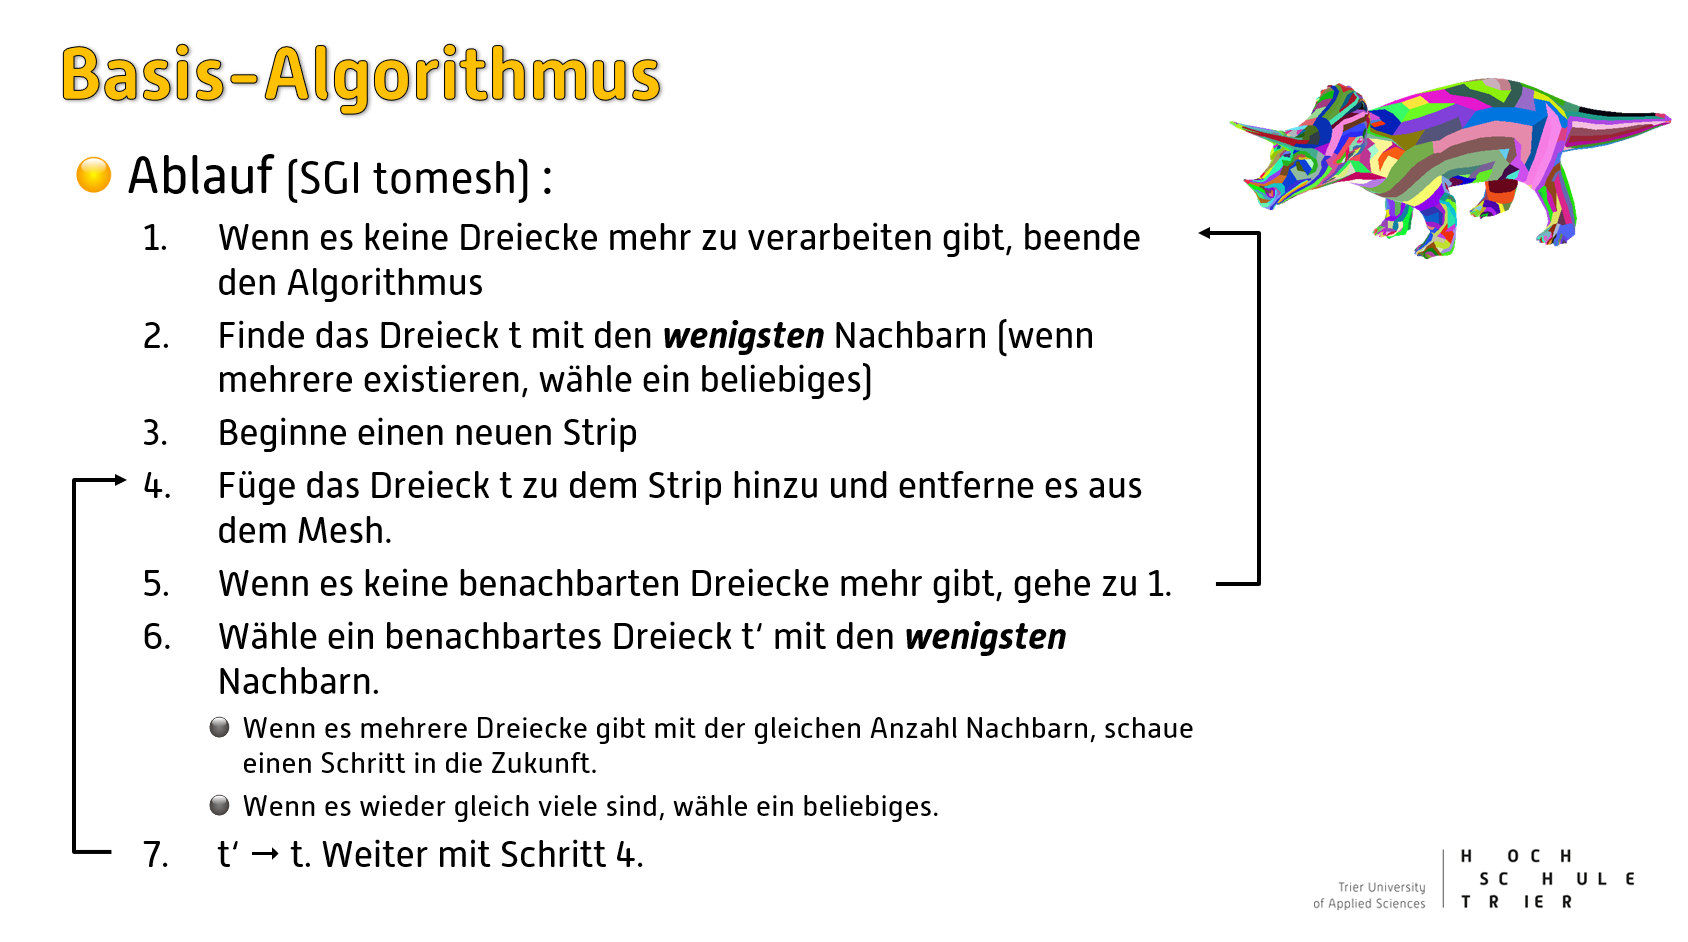
\includegraphics[scale = 0.3]{images/SGI-tomesh.PNG}
    \caption{Ablauf - SGI tomesh}
	\label{fig:SGI}
\end{figure} 
\hfil \break
Hier sind die wesentlichen Schritte und eine detaillierte Erklärung des
Algorithmus.
\begin{enumerate}
	\item \textbf{Initialisierung:} 
	\\
	Zu Beginn wird ein Vektor \lstinline{std::vector<int> triangle_indices} mit
	Indizes initialisiert, indem er inkrementell mit natürlichen Zahlen
	gefüllt wird. Diese Indizes repräsentieren die Indizes der Dreiecke im
	Vektor \lstinline{std::vector<Triangle> faces}.
	\\
	\item \textbf{Initialisierung der Nachbarn:} 
	\\
	Die Methode \lstinline{void initTriagleNeighbors()} wird aufgerufen, um das Attribut \break
	\lstinline{std::map<int, vector<int>> triangle_neighbors_indices} zu initialisieren.
	Diese Methode geht durch alle Dreiecke durch und speichert jeweils alle
	nicht-bearbeiteten Nachbardreiecke des jeweiligen Dreiecks in einen Vektor
	ab. Dieser Vektor wird an der entsprechenden Position in der Map
	gespeichert. Nicht-bearbeitete Dreiecke sind Dreiecke, die noch nicht Teil
	eines Strips sind. Ganz am Anfang gelten alle Dreiecke als nicht bearbeitet.
	\\
	\item \textbf{Hauptalgorithmus:} 
	\\
	Der Algorithmus beginnt eine äußere Schleife, die nur dann endet, wenn alle
	Dreiecke als bearbeitet markiert wurden. Dies wird überprüft, indem die
	Größe von \lstinline{std::unordered_set<int> processedTriangles} mit der Größe des
	Vektors \lstinline{triangle_indices} verglichen wird. Sollten die Größen gleich sein,
	kann geschlussfolgert werden, dass alle Dreiecke bearbeitet wurden.
	\\
	\item \textbf{Sortierung nach Nachbarn:} 
	\\
	Am Anfang jeder Iteration der äußeren Schleife werden die Indizes im Vektor
	\lstinline{triangle_indices} nach der Anzahl der nicht-bearbeiteten Nachbarn der
	jeweiligen Dreiecke in aufsteigender Reihenfolge sortiert, um
	sicherzustellen, dass in der aktuellen Iteration die Dreiecke mit den
	wenigsten Nachbarn immer vorne im Vektor stehen. Dieser Vektor wird jedes
	Mal neu sortiert, da sich die Anzahl der nicht-bearbeiteten Nachbardreiecke
	nach der Verarbeitung der Dreiecke unvorhersehbar ändert.
	\\
	\item \textbf{Beginn eines neuen Strips:} 
	\\
	Nachdem ein passendes Dreieck gefunden wurde, beginnt ein neuer Strip. Es
	wird die Variable \lstinline{std::vector<unsigned short> strip} deklariert, welche eine
	Liste der Vertices für einen Strip darstellt. Eine innere Schleife beginnt,
	die nur dann terminiert, wenn das aktive Dreieck \lstinline{active_triangle} keine
	weiteren nicht-bearbeiteten Nachbarn mehr hat. 
	\\
	\item \textbf{Hinzufügen von Dreiecken zu Strips:} 
	\\
	Direkt am Anfang der Schleife wird das Dreieck \lstinline{active_triangle} mit der
	Methode \lstinline{void addTriagleToStrip(const int targetIndex, vector<unsigned short>& strip)} 
	zum \break Strip hinzugefügt. Diese Methode schreibt die Vertices
	des übergebenen Dreiecks in den Vektor \lstinline{strip}. Falls \lstinline{strip} noch leer ist,
	werden die Vertices einfach hineingeschrieben, falls nicht, dann erfolgt
	eine Reihe von Überprüfungen:
	\\
	\begin{itemize}
	\item Es wird geprüft, ob die letzten zwei Vertices vom Strip im übergebenen
	Dreieck vorkommen. Falls ja, wird der Vertex in den Strip geschrieben,
	welcher nicht einer der beiden gemeinsamen Vertices war. 
	\\
	\item Sollte es nur einen gemeinsamen Vertex geben, kann davon ausgegangen
	werden, dass der zweite gemeinsame Vertex auf der drittletzten Stelle im
	Strip steht. In diesem Fall wird ein sogenannter Swap vorgenommen. Dabei wird das
	drittletzte Element des Strips kopiert und zwischen dem vorletzten und
	letzten Element eingefügt.
	\end{itemize} 
	
	\item \textbf{Wahl eines neuen Nachbardreiecks:} 
	\\
	Nach dem Abschluss der \lstinline{addTriagleToStrip}-Methode wird ein Nachbardreieck von
	\lstinline{active_triangle} gewählt, das die wenigsten Nachbarn hat und noch nicht
	bearbeitet wurde. Dazu wird der passende Vektor mit Nachbardreiecken aus der
	Map \lstinline{triangle_neighbors_indices} genommen und nach der Anzahl der
	nicht-bearbeiteten Nachbarn der jeweiligen Dreiecke in aufsteigender
	Reihenfolge sortiert.
	Falls es mehrere Dreiecke mit der gleichen Anzahl an Nachbarn gibt, werden die
	Nachbarn der Nachbarn (Nachbarn zweiten Grades) verglichen. Das Dreieck mit
	der kleinsten Summe der Nachbarn zweiten Grades wird zum neuen
	\lstinline{active_triangle}. 
	\\
	\item \textbf{Abschluss der Iteration:} 
	\\
	Nachdem ein kompletter Strip erstellt wurde und \lstinline{active_triangle} keine
	weiteren Nachbarn mehr hat, wird die innere Schleife verlassen. Der erzeugte
	Strip wird zum Vektor \lstinline{std::vector<vector<unsigned short>> strips}
	hinzugefügt, welcher eine Ansammlung von Strips darstellt. 
	\\
	\item \textbf{Fortsetzung der äußeren Schleife:} 
	\\
	Die äußere Schleife wird fortgesetzt, indem ein neues Dreieck mit den
	wenigsten nicht-bearbeiteten Nachbarn erneut gewählt und ein neuer Strip
	begonnen wird. Dieser Prozess wird so lange wiederholt, bis alle Dreiecke
	als bearbeitet markiert wurden. 
	\\
\end{enumerate}

\chapter{Implementierung des Strip-Zeichners}

Der Code, der für das Zeichnen von Strips zuständig ist, befindet sich in der
Methode \lstinline{void Mesh3D::draw()} in der Datei \lstinline{Mesh3d_render.cpp}. Diese Methode
verarbeitet und zeichnet die Strips der 3D-Mesh-Daten, die in der Mesh3D-Klasse
gespeichert sind. Die folgende detaillierte Beschreibung erklärt die
Funktionsweise dieser Methode.
\\
\\
Zu Beginn der Methode wird der Zufallszahlengenerator der Standardbibliothek
initialisiert. Dazu wird der Seed des Generators auf 0 gesetzt, um
sicherzustellen, dass die Farben bei jedem Aufruf der Methode \lstinline{draw()} konsistent
und wiederholbar sind. Dies bedeutet, dass trotz der zufälligen Natur der
Farbwerte die gleiche Farbe für denselben Strip bei jedem Methodenaufruf
verwendet wird. 
\\
\\
Es wird eine Zählvariable \lstinline{int counter} deklariert und auf 0 initialisiert. Diese
Variable dient dazu, die Anzahl der gezeichneten Strips während der
Schleifeniterationen zu zählen. Diese Zählung wird verwendet, um die maximale
Anzahl der zu zeichnenden Strips zu begrenzen, die durch die Konstante
\lstinline{strip_amount_limit} definiert ist.
\\
\\
Die Methode beginnt dann mit einer äußeren Schleife, die über alle Strip-Daten
iteriert. Der Schleifenmechanismus bricht ab, wenn die Anzahl der gezeichneten
Strips die festgelegte Grenze (\lstinline{strip_amount_limit}) erreicht. Dies stellt sicher,
dass nicht mehr Strips gezeichnet werden als zulässig.
\\
\\
Innerhalb der Schleife wird eine zufällige Farbe für den aktuellen Strip
generiert. Dies erfolgt durch Erzeugung von drei float-Werten \lstinline{r}, \lstinline{g} und \lstinline{b}, die
die RGB-Farben repräsentieren. Diese Werte werden durch die Division der vom
Zufallszahlengenerator zurückgegebenen Werte durch \lstinline{RAND_MAX} berechnet. Dies
sorgt dafür, dass die Werte im Bereich [0, 1] liegen, was der Farbdarstellung in
OpenGL entspricht. Die Funktion \lstinline{glColor3f(r, g, b)} wird verwendet, um diese
Farbe für den aktuellen Strip festzulegen.
\\
\\
Anschließend wird der Strip gezeichnet. Dies beginnt mit dem Aufruf von \break
\lstinline{glBegin(GL_TRIANGLE_STRIP)}, welcher OpenGL mitteilt, dass ein neuer Strip
gezeichnet wird. Innerhalb einer inneren Schleife werden die Indizes des
aktuellen Strips durchlaufen. Für jeden Index wird der entsprechende Vertex aus
dem \lstinline{vertices}-Array geladen und dessen Koordinaten an die GPU übergeben, indem
\lstinline{glVertex3f(float x, float y, float z)} aufgerufen wird.
\\
\\
Sobald alle Vertices für den aktuellen Strip verarbeitet wurden, wird die innere
Schleife beendet, und mit \lstinline{glEnd()} wird der Strip abgeschlossen und gezeichnet.
Die Zählvariable \lstinline{counter} wird inkrementiert, und die äußere Schleife fährt mit
dem nächsten Strip fort, bis entweder alle Strips gezeichnet wurden oder die
Grenze \lstinline{strip_amount_limit} erreicht ist.
\\
\\
Zusammengefasst, bereitet die Methode \lstinline{draw()} die Farbwerte vor, verwendet
OpenGL-Funktionen zum Zeichnen der Strips und sorgt durch die Zählvariable
dafür, dass nur eine begrenzte Anzahl von Strips gezeichnet wird. Die Verwendung
eines festen Seeds für den Zufallszahlengenerator sorgt dafür, dass die Farben
konsistent bleiben, während der Code in der Schleife die Strips effizient an die
GPU sendet und zeichnet.
\chapter{Implementierung der Steuerung und der GUI}

Die Methode \lstinline{renderGui()} und die Methode \lstinline{keyEvent(unsigned char key, int x, int y)} 
sind zentrale Bestandteile der Benutzeroberfläche und Steuerung für das
\lstinline{ViewerWindow}-Objekt. Im Folgenden wird detailliert beschrieben, wie diese
Methoden implementiert sind und welche Aufgaben sie erfüllen.
\\
\\
Die Methode \lstinline{renderGui()} ist verantwortlich für die Darstellung und
Aktualisierung der grafischen Benutzeroberfläche unter Verwendung von
ImGui, einer weit verbreiteten und leistungsfähigen Bibliothek für sofortige
GUI-Entwicklung (siehe \href{https://github.com/ocornut/imgui}{ImGui}). Diese Methode verwaltet die Benutzeroberfläche,
die dem Nutzer ermöglicht, verschiedene Interaktionen und Einstellungen
vorzunehmen.
\\
\begin{enumerate}
    \item \textbf{Ladefenster:}
    \\
    Wenn der \lstinline{isLoading}-Status auf true gesetzt ist, zeigt die Methode
    ein Ladefenster an, das den Benutzer darüber informiert, dass eine Aktion (wie
    das Laden eines neuen Meshes) im Gange ist. Dies geschieht durch den Aufruf von
    \lstinline{ImGui::Begin()} mit entsprechenden Flags, um das Fenster ohne Titel, Größe und
    Bewegung anzuzeigen. \lstinline{ImGui::Text()} wird verwendet, um den Ladehinweis
    darzustellen.
    \\
    \item \textbf{Haupt-Benutzeroberfläche:} 
    \\ 
    Sobald \lstinline{isLoading} auf false
    gesetzt ist, zeigt die Methode die Haupt-GUI an, die mehrere Abschnitte
    enthält: 
    \\
    \begin{itemize}
        \item 
        Unter dem Abschnitt 'Control' wird dem Benutzer erklärt, welche
        Tastenkombinationen zur Steuerung der Anzahl der anzuzeigenden Strips
        verwendet werden können. Die Beschreibungen dieser Steuerungen werden
        durch \lstinline{ImGui::Text()} bereitgestellt.
        \\
        \item 
        Im Abschnitt 'Mesh' kann der Benutzer zwischen verschiedenen
        Mesh-Dateien auswählen. Hierzu wird \lstinline{ImGui::BeginCombo()}
        verwendet, um ein Dropdown-Menü zu erstellen. Die Auswahl wird durch
        \lstinline{ImGui::Selectable()} ermöglicht, wobei die Variable
        \lstinline{selectedIndex} die Auswahl speichert. \\
        \item 
        Im Abschnitt 'Info' werden verschiedene Informationen über das aktuelle
        Mesh angezeigt. Dazu gehören die Anzahl der einzigartigen Vertices, der
        Dreiecksflächen und der Strips sowie die Anzahl und Einsparungen von
        Vertices, die an die GPU gesendet wurden. Berechnungen zur Anzahl der
        gesparten Vertices werden durchgeführt, und die Ergebnisse werden
        mittels \lstinline{ImGui::Text()} angezeigt. 
        \\
        \item 
        Ein Button mit der Beschriftung 'Process' ermöglicht das
        Laden eines neuen Meshes. Beim Klicken auf diesen Button wird der Status
        \lstinline{isLoading} auf true gesetzt und ein neuer Thread gestartet, der das Mesh
        aus einer .obj-Datei lädt. Der alte Mesh wird durch das neue ersetzt,
        und \lstinline{isLoading} wird auf false zurückgesetzt, sobald der Ladevorgang
        abgeschlossen ist.
    \end{itemize} 
    \hfil \break
    \item \textbf{Rendering und Abschluss:} 
    \\ 
    Nach der Erstellung und Aktualisierung der GUI wird \lstinline{ImGui::Render()}
    aufgerufen, um die GUI zu rendern, und \lstinline{ImGui_ImplOpenGL3_RenderDrawData()}
    wird verwendet, um die gerenderten GUI-Daten mit OpenGL anzuzeigen.
\end{enumerate}
\hfil \break
Die Methode \lstinline{keyEvent(unsigned char key, int x, int y)} wurde angepasst, um
Tastatureingaben zu verarbeiten und entsprechende Änderungen in der Anzeige der
Strips vorzunehmen. Der Parameter \lstinline{key} gibt die gedrückte Taste an, und basierend
auf diesem Wert wird eine der folgenden Aktionen ausgeführt:
\\
\begin{itemize}
    \item Wenn die Taste '1' gedrückt wird, wird die Anzahl der anzuzeigenden Strips
    um eins reduziert, vorausgesetzt, die Anzahl ist nicht bereits auf 0 reduziert.
    \\
    \item Bei Drücken der Taste '2' wird die Anzahl der anzuzeigenden Strips um eins
    erhöht, sofern sie nicht bereits die maximale Anzahl der verfügbaren Strips
    erreicht hat.
    \\
    \item Wenn die Taste '3' gedrückt wird, wird entweder die Anzahl
    der anzuzeigenden Strips auf 0 gesetzt (was alle Strips ausblendet) oder auf die
    Gesamtanzahl der verfügbaren Strips, um alle anzuzeigen.
\end{itemize}

\chapter{Weitere Anpassungen}

In diesem Kapitel werden die Änderungen an weiteren Code-Stellen erläutert.
\\
\begin{itemize}
    \item 
    In der \lstinline{main.cpp} wurden Anpassungen vorgenommen, um die
    Callback-Funktionen für das Fenster-Management zu aktualisieren und die
    Interaktionen zwischen ImGui und der Hauptfensterinstanz zu ermöglichen. Die
    Funktionen \lstinline{reshape}, \lstinline{keyboard}, \lstinline{mouse} und
    \lstinline{move} wurden so modifiziert, dass sie sowohl die
    ImGui-spezifischen Anforderungen erfüllen als auch die entsprechenden
    Methoden des ViewerWindow-Objekts aufrufen. 
    \\
    Zusätzlich wurde ImGui in der
    \lstinline{main()}-Funktion initialisiert, indem die ImGui-Version
    überprüft, ein ImGui-Kontext erstellt, das Dark-Theme angewendet und die
    ImGui-Backends für GLUT und OpenGL3 konfiguriert wurden.
    \\
    \item 
    In der \lstinline{CGlutWindow}-Klasse wurden spezifische Anpassungen für die Integration
    von ImGui vorgenommen. Beim Destruktor der Klasse wurde der Code hinzugefügt, um ImGui-Ressourcen zu
    bereinigen.
    \\
    Zusätzlich wurde in der \lstinline{renderFrame()}-Methode der Code ergänzt, um einen
    neuen ImGui-Frame zu beginnen und zu rendern. 
    \\
    \item 
    Alle Funktionalitäten zum Einlesen und Verarbeiten von Normalen und
    Texturkoordinaten wurden entfernt, da sie nicht mehr benötigt werden.
    \\
    \item 
    Entsprechende Header-Dateien wurden angepasst, um die neuen Funktionalitäten zu integrieren.
\end{itemize}
\chapter{Zusammenfassung und Ausblick}

In diesem Kapitel soll die Arbeit noch einmal kurz zusammengefasst werden. Insbesondere sollen die wesentlichen Ergebnisse Ihrer Arbeit herausgehoben werden. Erfahrungen, die z.B. Benutzer mit der Mensch-Maschine-Schnittstelle gemacht haben oder Ergebnisse von Leistungsmessungen sollen an dieser Stelle präsentiert werden. Sie können in diesem Kapitel auch die Ergebnisse oder das Arbeitsumfeld Ihrer Arbeit kritisch bewerten. Wünschenswerte Erweiterungen sollen als Hinweise auf weiterführende Arbeiten erwähnt werden.



\end{document}
